\section{Girolamo Giacomino
Gorgonzola}\label{girolamo-giacomino-gorgonzola}

Tags: NPC Alias: GGG Creatore: Davide Ispirazione: Geronimo Stilton; JJ
Jameson Luogo: Kos

\section{Girolamo Giacomino
Gorgonzola}\label{girolamo-giacomino-gorgonzola-1}

\begin{center}\rule{0.5\linewidth}{0.5pt}\end{center}

\begin{figure}
\centering
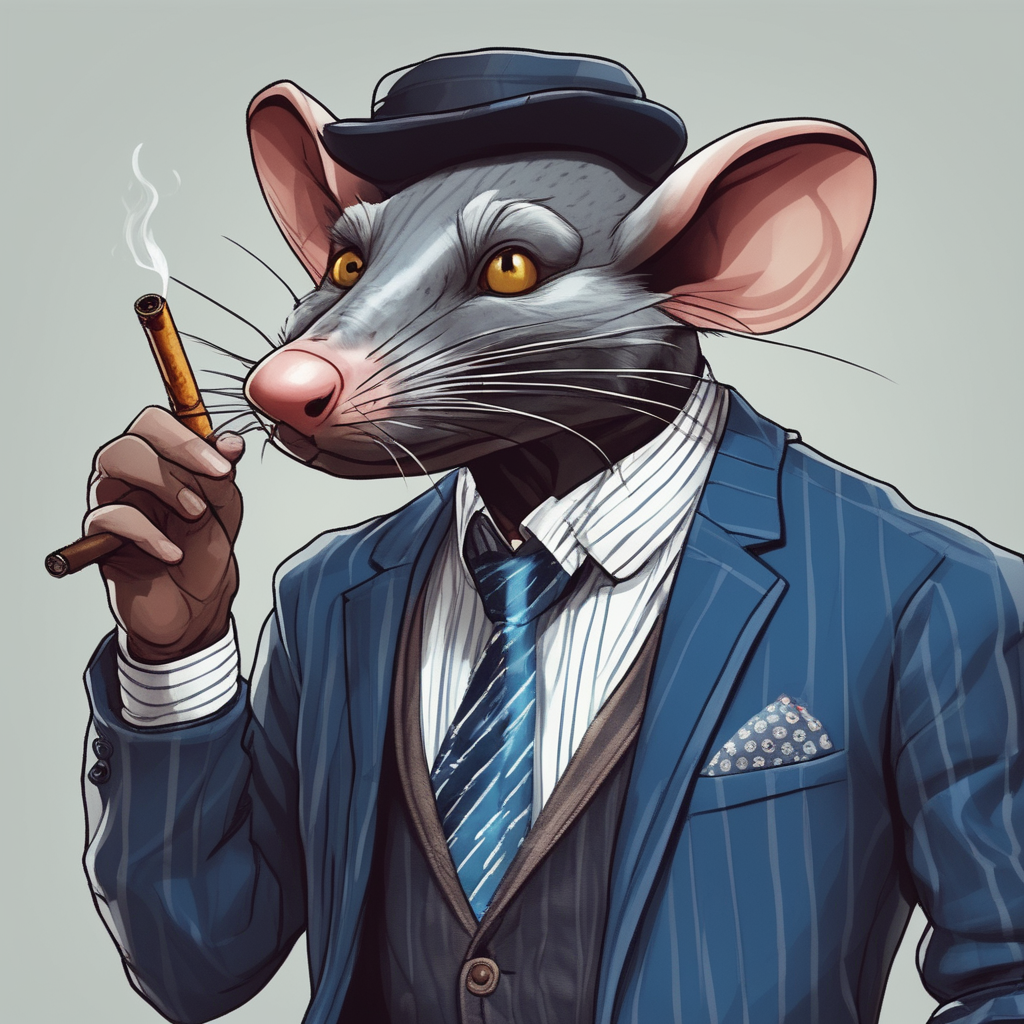
\includegraphics{create-an-image-of-a-human-folk-a-fantasy-race-with-humankind-features-resembling-a-rat-he-has-a-st.png}
\caption{create-an-image-of-a-human-folk-a-fantasy-race-with-humankind-features-resembling-a-rat-he-has-a-st.png}
\end{figure}

Informazioni Generali

Età: 44

Data di nascita: 26/12/1978

Luogo di nascita: Kos

Razza: Ratfolk

Professione: Giornalista

Alias: Un topo, anzi un tipo

\begin{center}\rule{0.5\linewidth}{0.5pt}\end{center}

\subsection{1. Descrizione Generale}\label{descrizione-generale}

\begin{center}\rule{0.5\linewidth}{0.5pt}\end{center}

\begin{figure}
\centering
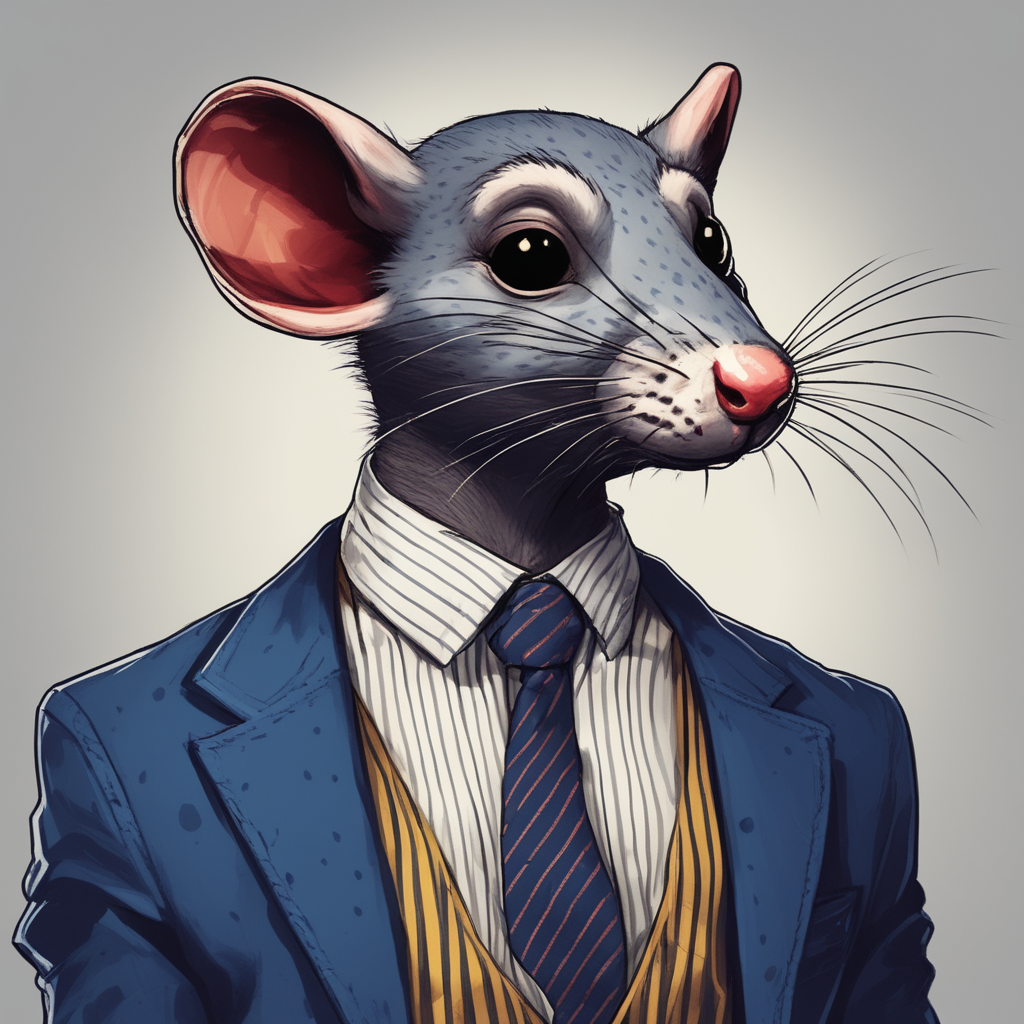
\includegraphics{create-an-image-of-a-human-folk-a-fantasy-race-with-humankind-features-resembling-a-rat-he-has-a-st-3.png}
\caption{create-an-image-of-a-human-folk-a-fantasy-race-with-humankind-features-resembling-a-rat-he-has-a-st-3.png}
\end{figure}

Girolamo Gorgonzola è una figura rispettata e ammirata nel mondo del
giornalismo di Valtara, un individuo con una personalità affascinante e
una profonda passione per l'avventura, la cultura e la verità.

\begin{quote}
``Garantito al formaggio!''
\end{quote}

\subsection{2. Biografia}\label{biografia}

\begin{center}\rule{0.5\linewidth}{0.5pt}\end{center}

\subsubsection{2.1 Infanzia e istruzione}\label{infanzia-e-istruzione}

\begin{center}\rule{0.5\linewidth}{0.5pt}\end{center}

Girolamo Gorgonzola, un nativo di Kos, ha trascorso la sua infanzia
immerso in libri e racconti avventurosi. Fin da piccolo, dimostrava una
curiosità insaziabile e un'innata passione per le storie. Passava ore
nelle biblioteche locali, leggendo romanzi d'avventura e inseguendo
misteri. Questi primi anni hanno forgiato la sua immaginazione e nutrito
il desiderio di esplorare il mondo.

\subsubsection{2.2 Gioventù e Passione per
l'Investigazione}\label{gioventuxf9-e-passione-per-linvestigazione}

\begin{center}\rule{0.5\linewidth}{0.5pt}\end{center}

Mentre frequentava la scuola, Girolamo iniziò a distinguersi per le sue
doti investigative e il suo talento nella scrittura. Organizzava gruppi
di amici per risolvere piccoli enigmi e misteri locali, creando le basi
per la sua futura carriera. Durante questo periodo, sviluppò anche una
forte amicizia con un compagno ratfolk, un elfo esperto di crimine, e un
folletto autore di romanzi gialli, con i quali condivideva una passione
comune per il mistero e l'avventura.

\subsubsection{2.3 Interessi Personali}\label{interessi-personali}

\begin{center}\rule{0.5\linewidth}{0.5pt}\end{center}

Oltre alla sua carriera giornalistica, Girolamo aveva un hobby segreto:
collezionare antichi manoscritti e mappe dei tempi antichi. Questi
documenti preziosi rappresentavano il suo amore per la storia e
l'archeologia, e spesso faceva spedizioni per cercare artefatti nascosti
in luoghi misteriosi. La sua casa era una testimonianza vivente di
queste scoperte.

\subsubsection{2.4 Vita Familiare}\label{vita-familiare}

\begin{center}\rule{0.5\linewidth}{0.5pt}\end{center}

Girolamo ha formato una famiglia con una compagna ratfolk, Isabella,
anch'essa una giornalista di talento. La coppia ha avuto tre figli, che
crescono con una curiosità simile per il mondo che circonda Kos. La vita
familiare ha introdotto sfide e responsabilità aggiuntive, ma Girolamo
ha sempre cercato di bilanciare il lavoro e la famiglia. Spesso, le sue
storie più toccanti riguardavano temi familiari e comunitari,
riflettendo la sua profonda connessione con la sua città e i suoi cari.

\subsection{3. Carriera}\label{carriera}

\begin{center}\rule{0.5\linewidth}{0.5pt}\end{center}

\subsubsection{3.1 Inizio al ``Pane
Quotidiano''}\label{inizio-al-pane-quotidiano}

\begin{center}\rule{0.5\linewidth}{0.5pt}\end{center}

Dopo aver completato gli studi in giornalismo, Girolamo ha iniziato la
sua carriera come giovane reporter per il ``Pane Quotidiano'', la
principale testata giornalistica di Kos, che però opera in tutta
Valtara. Ha scritto articoli su eventi locali e storie di comunità,
guadagnandosi gradualmente il rispetto dei suoi colleghi e dei lettori.
Durante questi anni, ha sviluppato il suo stile di scrittura unico e
coinvolgente.

\subsubsection{3.2 Avanzamento e Raggiungimento della
Direzione}\label{avanzamento-e-raggiungimento-della-direzione}

\begin{center}\rule{0.5\linewidth}{0.5pt}\end{center}

Con il passare del tempo, Girolamo è avanzato nella redazione e ha
ottenuto il titolo di direttore del ``Pane Quotidiano''. Ha utilizzato
la sua posizione per promuovere l'onestà e l'integrità nel giornalismo,
impegnandosi a raccontare la verità e a svelare gli scandali. Il suo
stile di scrittura vivace e coinvolgente ha catturato l'attenzione di
molte persone in tutta la regione di Valtara. La sua carriera
giornalistica è stata contraddistinta da una serie di storie rivelatrici
e avvincenti, spesso basate sulla sua passione per l'investigazione e
l'amore per le storie avventurose.

\subsection{4. Personalità}\label{personalituxe0}

\begin{center}\rule{0.5\linewidth}{0.5pt}\end{center}

Girolamo Gorgonzola è noto per la sua personalità brillante e
carismatica. È un individuo appassionato, con una profonda sete di
conoscenza e un amore innato per le storie. La sua curiosità è
contagiosa e ispira chiunque lo incontri.

È un giornalista di grande integrità, che crede fermamente nella
responsabilità dei media nel garantire una società giusta e trasparente.
È determinato a fare luce sugli eventi misteriosi e a svelare la verità,
anche quando questo significa affrontare rischi.

La sua vita familiare, caratterizzata da amore e sostegno reciproco, è
fondamentale per la sua stabilità e influenza positivamente il suo
approccio al lavoro. È anche un uomo di cultura, appassionato di storia
e archeologia, che ama esplorare il passato alla ricerca di segreti
nascosti.

Complessivamente, Girolamo Gorgonzola è una figura rispettata e ammirata
nel mondo del giornalismo di Valtara, un individuo con una personalità
affascinante e una profonda passione per l'avventura, la cultura e la
verità.

\subsection{A. Coinvolgimenti in eventi
recenti}\label{a.-coinvolgimenti-in-eventi-recenti}

\begin{center}\rule{0.5\linewidth}{0.5pt}\end{center}

\href{Untitled\%209eb2c6b2c8d14a40a96386c65efaf53b.csv}{}

\subsection{B. Aggiornamenti}\label{b.-aggiornamenti}

\begin{center}\rule{0.5\linewidth}{0.5pt}\end{center}

\href{Untitled\%20599168486376461b8d09a83dbcfd3ceb.csv}{}

\subsection{C. Galleria Immagini}\label{c.-galleria-immagini}

\begin{figure}
\centering
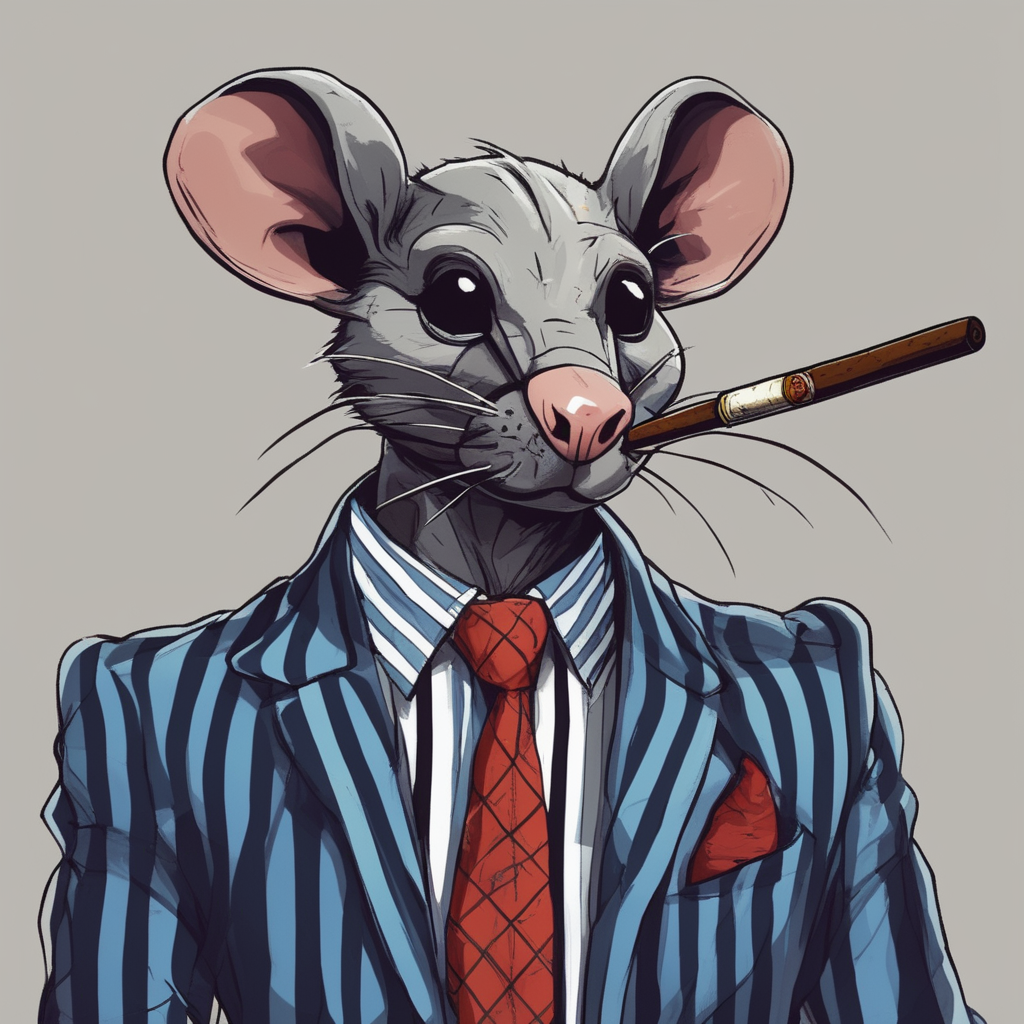
\includegraphics{create-an-image-of-a-human-folk-a-fantasy-race-with-humankind-features-resembling-a-rat-he-has-a-st-2.png}
\caption{Classica foto di Girolamo che compare alla fine degli articoli
che firma}
\end{figure}

Classica foto di Girolamo che compare alla fine degli articoli che firma
